\chapter{Background}
\label{cap:background}

\section{Analisi del Malware}
Con l'escalation della complessità delle minacce informatiche, è diventato cruciale sviluppare metodologie avanzate per l'analisi dei malware. Il termine "malware", abbreviazione di \emph{malicious software} (software maligno), raggruppa una varietà di programmi progettati per infiltrarsi, danneggiare o compromettere sistemi informatici senza il consenso dell'utente. L'analisi dei malware è il processo sistematico di esame e comprensione di questi software per determinarne il funzionamento, l'origine, gli obiettivi e le vulnerabilità sfruttabili per una difesa efficace.

L'analisi dei malware si articola principalmente in due categorie: analisi statica e analisi dinamica.

\subsection{Analisi Statica}
L'analisi statica del malware implica l'esame del codice sorgente o dei file binari senza eseguirli, permettendo agli analisti di identificare caratteristiche intrinseche del malware. Questo metodo comprende l'analisi di stringhe di testo, importazioni di API, strutture di codice e pattern specifici che possono suggerire attività malevole. Strumenti quali disassemblatori (per esempio, IDA Pro) e decompilatori (come Ghidra) sono essenziali per facilitare questa analisi, convertendo il codice binario in una forma più leggibile e interpretabile.
Tuttavia, l'analisi statica incontra notevoli sfide. I creatori di malware adottano spesso tecniche di offuscamento e cifratura per mascherare il vero comportamento del codice, complicando l'interpretazione sia manuale che automatizzata. Tecniche come il packing, il polimorfismo e il metamorfismo sono esempi di metodi usati per aumentare la resistenza del malware all'analisi statica.
L'introduzione delle Generative Adversarial Networks (GAN) nell'analisi statica promette soluzioni innovative. Le GAN possono essere utilizzate per generare automaticamente campioni sintetici di malware, ampliando i dataset disponibili per l'addestramento dei modelli di machine learning. Questo approccio non solo arricchisce la varietà dei campioni analizzati ma migliora anche la comprensione delle diverse varianti e tecniche di evasione impiegate dai creatori di malware. Inoltre, le GAN possono essere sfruttate per affinare le tecniche di offuscamento, consentendo agli analisti di testare la robustezza degli strumenti di analisi statica contro nuove forme di malware.


\subsection{Analisi Dinamica}
L'analisi dinamica consiste nell'esecuzione del malware all'interno di un ambiente controllato, come una sandbox, per osservare il suo comportamento in tempo reale. Questo metodo consente di identificare azioni malevole quali modifiche al registro di sistema, creazione di file, comunicazioni di rete sospette e interazioni con altre applicazioni. A differenza dell'analisi statica, l'analisi dinamica può rivelare comportamenti malevoli non immediatamente discernibili dall'analisi del codice sorgente, specialmente quando il malware impiega tecniche di offuscamento o cifratura.

Nonostante la sua efficacia, l'analisi dinamica presenta delle limitazioni. Essa richiede risorse computazionali significative per eseguire i campioni di malware in ambienti isolati e per monitorarne le attività. Inoltre, alcuni malware sono capaci di riconoscere la presenza di ambienti di analisi e possono alterare il proprio comportamento per eludere la rilevazione, riducendo così l'efficacia dell'analisi.

Le Generative Adversarial Networks (GAN) possono migliorare l'analisi dinamica in vari modi. Per esempio, possono essere utilizzate per simulare ambienti di esecuzione più realistici, rendendo più difficile per il malware riconoscere e adattarsi all'ambiente di analisi. Inoltre, le GAN possono generare traffico di rete sintetico e scenari di attacco realistici, che aiutano gli analisti a testare e rafforzare le capacità di rilevamento delle sandbox. Infine, le GAN possono essere impiegate per creare modelli di comportamento dei malware, facilitando la previsione e l'identificazione di nuove varianti basate su schemi comportamentali precedentemente osservati.


\subsection{Visualizzazione del Malware}
La visualizzazione del malware è una tecnica avanzata che sfrutta rappresentazioni grafiche per facilitare l'analisi della struttura e del comportamento dei codici malevoli. Strumenti visivi quali diagrammi di flusso, grafici delle chiamate, mappe di rete e rappresentazioni grafiche delle interazioni tra i componenti sono ampiamente utilizzati in questo ambito. Questi strumenti aiutano gli analisti a identificare pattern ricorrenti, a riconoscere rapidamente le attività sospette e a comprendere le complesse relazioni intrinseche al codice.

Una rappresentazione visiva efficace può notevolmente accelerare il processo di analisi, consentendo agli analisti di scoprire anomalie e comportamenti insidiosi che potrebbero non emergere chiaramente attraverso l'analisi testuale o statica. Per esempio, un grafo delle chiamate API può rivelare sequenze anomale di chiamate indicative di attività di Command and Control (C\&C) o di esfiltrazione di dati.

L'integrazione delle Generative Adversarial Networks (GAN) nella visualizzazione del malware può innalzare il livello delle rappresentazioni a nuove vette di interattività e avanzamento. Le GAN sono capaci di generare visualizzazioni sintetiche che simulano scenari di attacco realistici, arricchendo così la comprensione degli analisti sulle possibili modalità di infiltrazione e propagazione del malware. Inoltre, l'uso delle GAN per creare visualizzazioni dinamiche, che si aggiornano in tempo reale con l'acquisizione di nuovi dati durante l'analisi dinamica, migliora notevolmente la capacità di rilevare anomalie e di interpretare le complesse dinamiche interne al codice, agevolando una risposta più tempestiva ed efficace contro le minacce emergenti.
\newpage
\begin{figure}[ht]
    \centering
    \begin{minipage}{0.45\textwidth}
        \centering
        
\includegraphics[width=0.9\linewidth]{images/adware.png}
        \label{fig:adware}
    \end{minipage}\hfill
    \begin{minipage}{0.45\textwidth}
        \centering
        
\includegraphics[width=0.9\linewidth]{images/spyware.png}
        \label{fig:spyware}
    \end{minipage}
\end{figure}
\captionof{figure}{Immagini in scala di grigi di malware di famiglia Adware e Spyware}

\subsection{Machine Learning}

Il \emph{machine learning} (ML) ha rivoluzionato il campo della sicurezza informatica, fornendo strumenti avanzati per la rilevazione e la classificazione del malware. Gli algoritmi di ML, sia supervisionati che non supervisionati, vengono addestrati su dataset di malware noti per identificare nuove minacce in modo automatico e scalabile. Tecniche quali alberi decisionali, macchine a vettori di supporto (SVM), metodi di clustering e reti neurali sono ampiamente impiegate in questo ambito.

Gli algoritmi di ML supervisionati richiedono dataset etichettati, nei quali ogni campione è classificato come benigno o malevolo. Tali algoritmi apprendono a distinguere pattern e caratteristiche specifiche del malware, permettendo loro di classificare nuovi campioni basandosi sulle informazioni acquisite. Al contrario, gli algoritmi di ML non supervisionati operano senza etichette predefinite, identificando autonomamente cluster di comportamenti simili, il che facilita la scoperta di nuove varianti di malware non ancora classificate.

Nonostante questi vantaggi, il ML tradizionale può essere limitato dalla qualità e dalla quantità dei dati disponibili. La carenza di campioni di malware etichettati può ridurre l'efficacia degli algoritmi di ML, compromettendo l'identificazione di nuove minacce. Inoltre, i modelli di ML possono essere vulnerabili a tecniche di evasione, nelle quali i creatori di malware modificano i loro campioni per eludere la rilevazione.

\subsection{Deep Learning}

Il \emph{deep learning} (DL), una branca avanzata del machine learning, sfrutta reti neurali profonde per modellare e riconoscere pattern complessi nei dati. Architetture come le reti neurali convoluzionali (CNN) e le reti neurali ricorrenti (RNN) sono particolarmente efficaci nell'analisi di malware, data la loro capacità di estrarre caratteristiche di alto livello dai campioni di codice. Le CNN sono rinomate per il loro eccellente riconoscimento di pattern spaziali, mentre le RNN sono ottimali per l'analisi di sequenze temporali di dati, rendendole strumenti ideali per il rilevamento di comportamenti sospetti nei flussi di dati.

Il DL ha ottenuto risultati notevoli nella classificazione e nella rilevazione di malware, anche quelli sconosciuti. Modelli di DL possono essere addestrati su vasti dataset di codici maligni e benigni per apprendere rappresentazioni complesse, che aiutano a differenziare tra codice malevolo e non. Inoltre, le tecniche di \emph{transfer learning} consentono di adattare modelli pre-addestrati a nuovi domini o varianti di malware, migliorando sia l'efficienza dell'addestramento sia la precisione delle predizioni.

L'introduzione delle \emph{Generative Adversarial Networks} (GAN) nel deep learning può ulteriormente amplificare questi successi. Le GAN possono essere utilizzate per generare nuovi campioni di malware che mettono alla prova i modelli di rilevazione esistenti, facilitando una continua evoluzione e miglioramento dei modelli di DL. Questo processo di \emph{adversarial training} rende i modelli di DL più robusti contro le tecniche di evasione utilizzate dai creatori di malware. In aggiunta, le GAN possono essere impiegate per creare rappresentazioni avanzate di dati di malware, potenziando la capacità dei modelli di DL di estrarre caratteristiche significative e di generalizzare a nuovi tipi di minacce.


\begin{figure}[ht]
    \centering
        \centering
        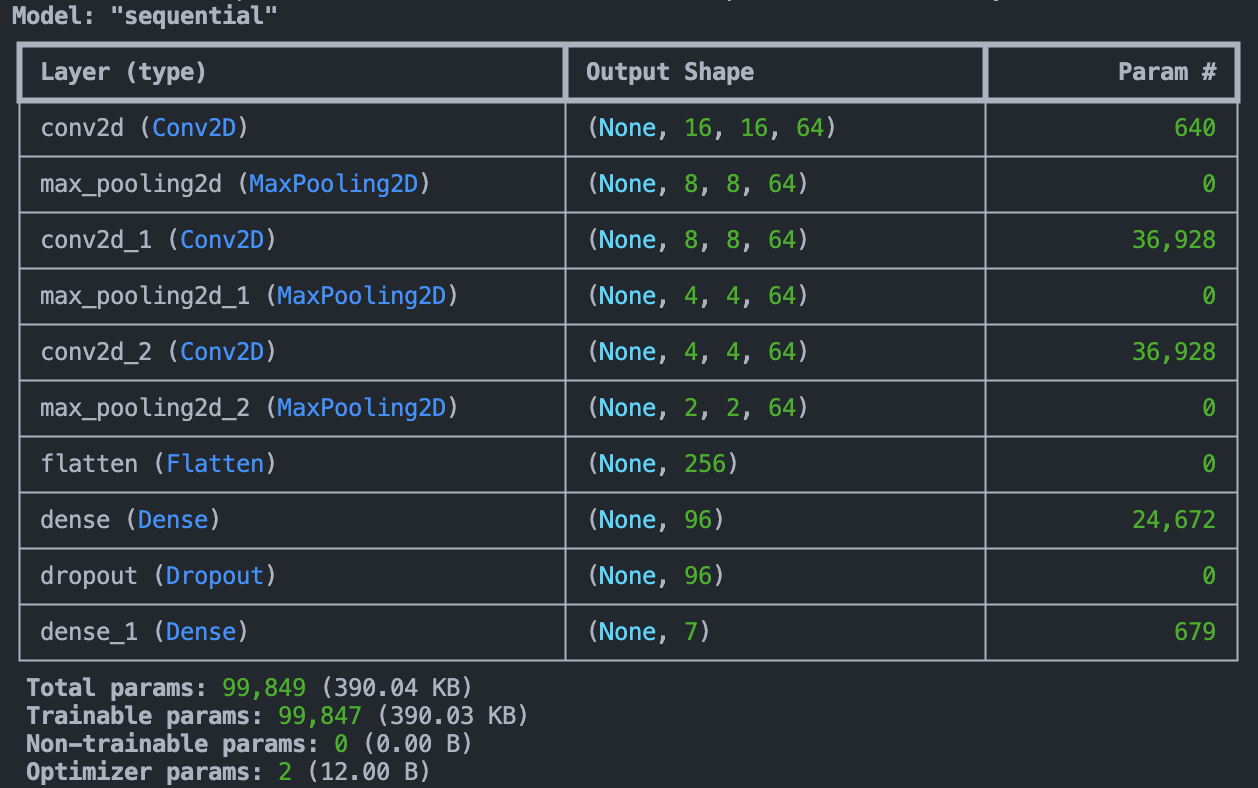
\includegraphics[width=0.8\linewidth]{images/cnn_architecture.png}
        \label{fig:cnn_architecture}
\end{figure}
\captionof{figure}{Architettura della rete neurale convoluzionale (CNN) utilizzata}

\subsection{Riproducibilità}

La riproducibilità è un principio cardinale nella ricerca scientifica, essenziale per garantire che i risultati ottenuti siano verificabili e replicabili da altri ricercatori. Nel campo dell'analisi del malware, ciò implica la disponibilità di dataset, codici sorgente, configurazioni di esperimenti e ambienti di esecuzione utilizzati negli studi, consentendo ad altri di validare i risultati, confrontare metodologie diverse e costruire su scoperte esistenti.

Tuttavia, la natura dinamica delle minacce informatiche può ostacolare la riproducibilità. I dataset di malware possono rapidamente diventare obsoleti con l'emergere di nuove varianti e tecniche di evasione. Le discrepanze negli ambienti di analisi, nelle configurazioni dei tool e nelle versioni del software possono altresì alterare i risultati degli esperimenti, rendendo ardua la replicazione esatta degli studi.

L'adozione delle \emph{Generative Adversarial Networks} (GAN) per generare dataset sintetici standardizzati può essere di grande aiuto nella condivisione e replicazione degli esperimenti. Le GAN sono in grado di produrre campioni di malware che riflettono le caratteristiche dei dataset originali ma introducono variazioni controllate per aumentare la diversità e rappresentatività. Questo metodo assicura che i dataset rimangano attuali e pertinenti anche di fronte a nuove minacce. Inoltre, le GAN possono essere utilizzate per simulare scenari di attacco complessi, facilitando la verifica delle metodologie in ambienti controllati e riproducibili.

La creazione di framework open-source che integrano GAN e altre tecnologie di analisi del malware può ulteriormente promuovere la trasparenza e la condivisione di conoscenze. Rendendo accessibili i codici sorgente e le configurazioni sperimentali, si permette ad altri ricercatori di replicare gli studi, identificare bias o limitazioni nei metodi esistenti e suggerire miglioramenti. Questo incoraggia una collaborazione più efficace all'interno della comunità scientifica per affrontare le sfide emergenti nel campo della sicurezza informatica.


\subsection{Explainability}

L'interpretabilità, o \emph{explainability}, dei modelli di machine learning e deep learning è fondamentale per comprendere come e perché questi modelli prendono specifiche decisioni. Nel campo della sicurezza informatica, è cruciale che gli analisti siano in grado di interpretare i risultati degli algoritmi di rilevazione del malware per prendere decisioni informate e comprendere le motivazioni dietro le segnalazioni di minacce. Tuttavia, modelli complessi come le reti neurali profonde spesso agiscono come "scatole nere", rendendo arduo discernere il ragionamento dietro le loro predizioni.

L'interpretabilità assume un'importanza particolare in contesti dove le decisioni devono essere giustificate, come in ambiti aziendali o legali, dove dimostrare la validità delle analisi è imprescindibile. Senza una chiara comprensione del funzionamento interno dei modelli, può essere difficile identificare errori o bias, limitando così la fiducia e l'adozione di queste tecnologie da parte di analisti e decision makers.

Le \emph{Generative Adversarial Networks} (GAN), nonostante siano strumenti generativi potenti, presentano notevoli sfide in termini di interpretabilità. Composte da due reti neurali — il generatore e il discriminatore — che competono tra loro, le GAN complicano il tracciamento e la comprensione dei processi interni che guidano la generazione dei campioni sintetici. Questa complessità può ostacolare la capacità di spiegare come e perché un campione di malware sintetico è stato generato in un determinato modo, o di distinguere le caratteristiche che separano un campione benigno da uno malevolo.

Per superare queste sfide, è vitale sviluppare metodi che aumentino la trasparenza nel processo decisionale delle GAN. Tecniche come l'analisi delle attivazioni interne, la visualizzazione delle rappresentazioni latenti e l'impiego di modelli intrinsecamente interpretabili possono migliorare significativamente l'interpretabilità delle GAN. Inoltre, l'adozione di approcci ibridi che combinano GAN con modelli più interpretabili può facilitare una migliore comprensione delle dinamiche interne, permettendo agli analisti di delineare le origini delle decisioni prese dai modelli generativi.

L'applicazione di tecniche di spiegazione post-hoc, come LIME (Local Interpretable Model-agnostic Explanations) o SHAP (SHapley Additive exPlanations), ai modelli di GAN offre un ulteriore strumento per fornire spiegazioni locali delle predizioni. Questi metodi aiutano a chiarire quali caratteristiche dei dati di input hanno maggiormente influenzato la generazione dei campioni, offrendo agli analisti insight preziosi per interpretare e validare i risultati.

La ricerca nell'ambito dell'\emph{explainable artificial intelligence} (XAI) sta sviluppando nuove strategie per rendere i modelli generativi più trasparenti e comprensibili. Integrare i principi di XAI nelle architetture delle GAN può portare alla creazione di modelli che non solo generano campioni realistici ma che forniscono anche spiegazioni dettagliate e comprensibili delle loro operazioni. Questo passo è fondamentale per incrementare la fiducia degli analisti nella tecnologia e promuovere un'adozione più ampia delle GAN nell'analisi del malware.

In conclusione, migliorare l'interpretabilità è un obiettivo cruciale per assicurare che le GAN e altri modelli avanzati di machine learning possano essere impiegati efficacemente e affidabilmente nell'analisi del malware. Una comprensione chiara e trasparente dei processi decisionali interni è essenziale per sfruttare appieno il loro potenziale e garantire la sicurezza e l'affidabilità delle analisi condotte.


%TODO aggiungere foto della heatmap 